\section{Preliminary Result}

\subsection{Workload characterization}



\begin{figure}[t]
    \centering
    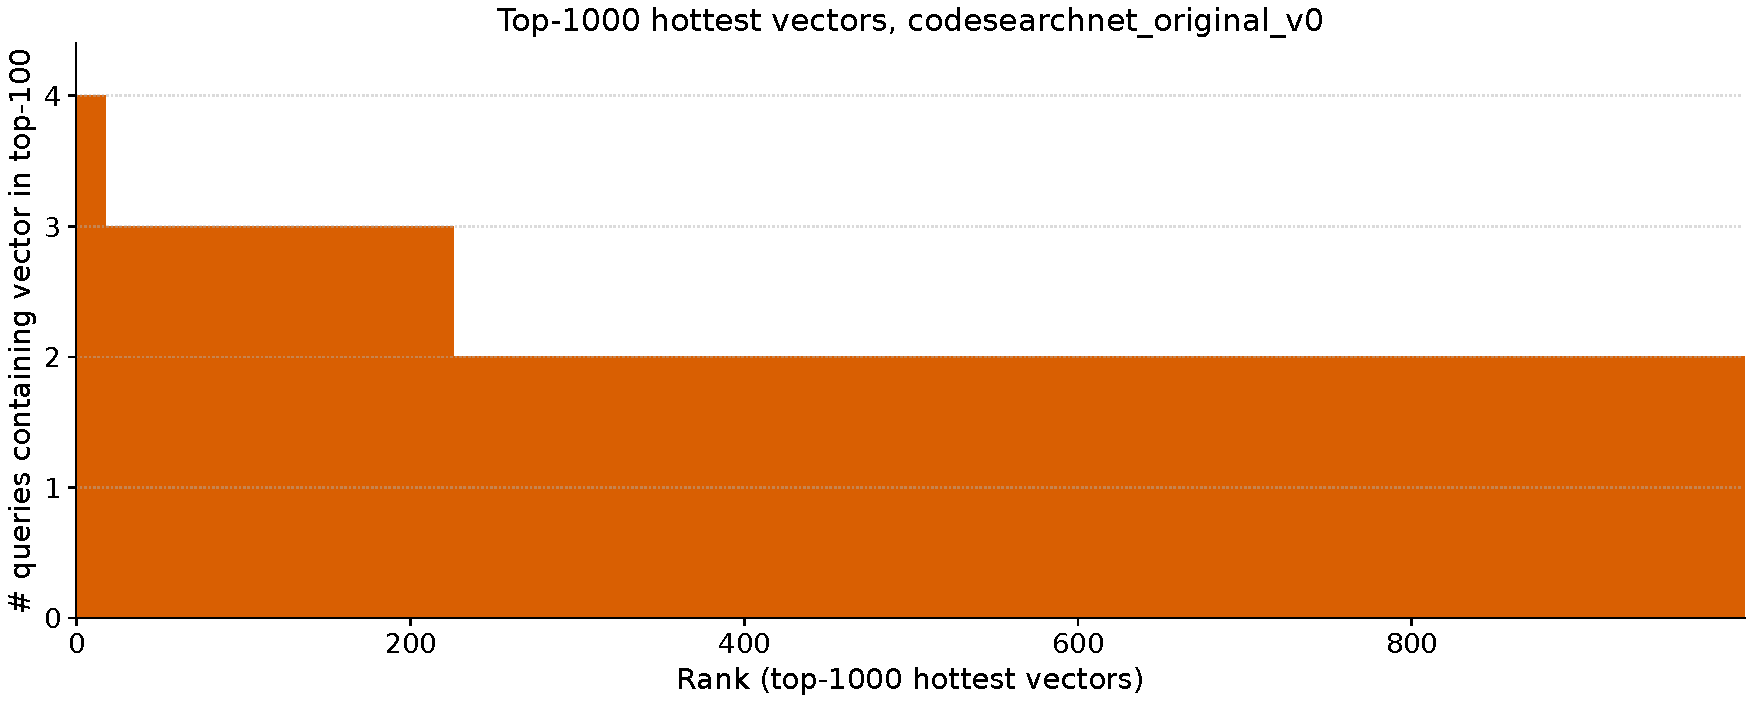
\includegraphics[width=\linewidth]{Figures/vector_hotness_top1000_codesearchnet_original_v0.pdf}
    \caption{Vector hotness for original, measured as the number of
    benchmark queries that include a given vector in their top-100
    ground-truth set.}
    \label{fig:hotness}
\end{figure}
\begin{figure}[t]
    \centering
    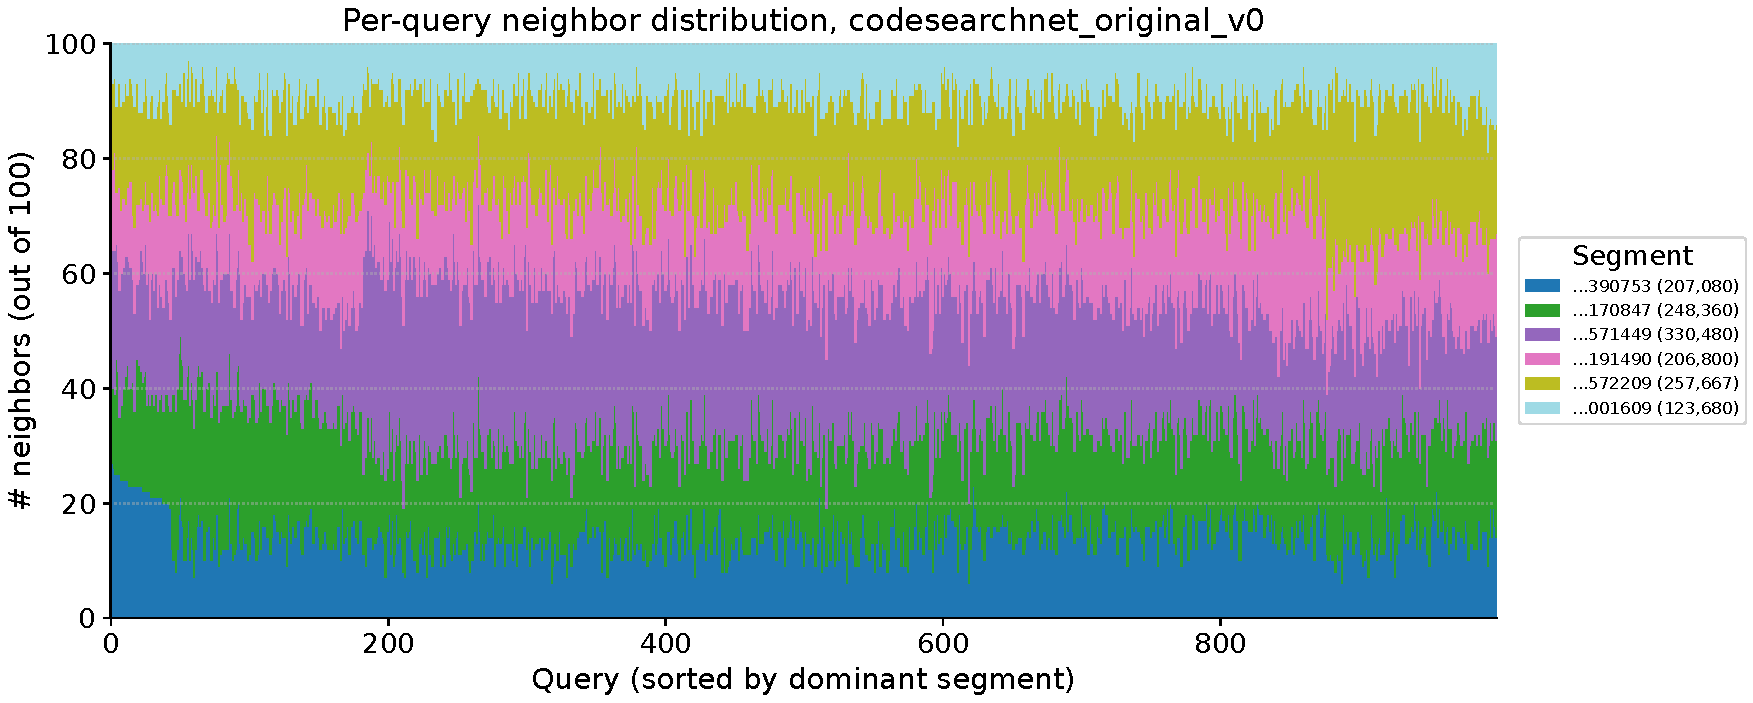
\includegraphics[width=\linewidth]{Figures/query_neighbor_segments_stacked_codesearchnet_original_v0.pdf}
    \caption{Per-query distribution of top-100 ground-truth neighbors
    across segments of the original collection. Each bar is a query,
    sorted by its dominant segment, each color is one segment. Most
    queries pull neighbors from several segments rather than a single
    hot one.}
    \label{fig:query-segments}
\end{figure}


\begin{figure}[t]
    \centering
    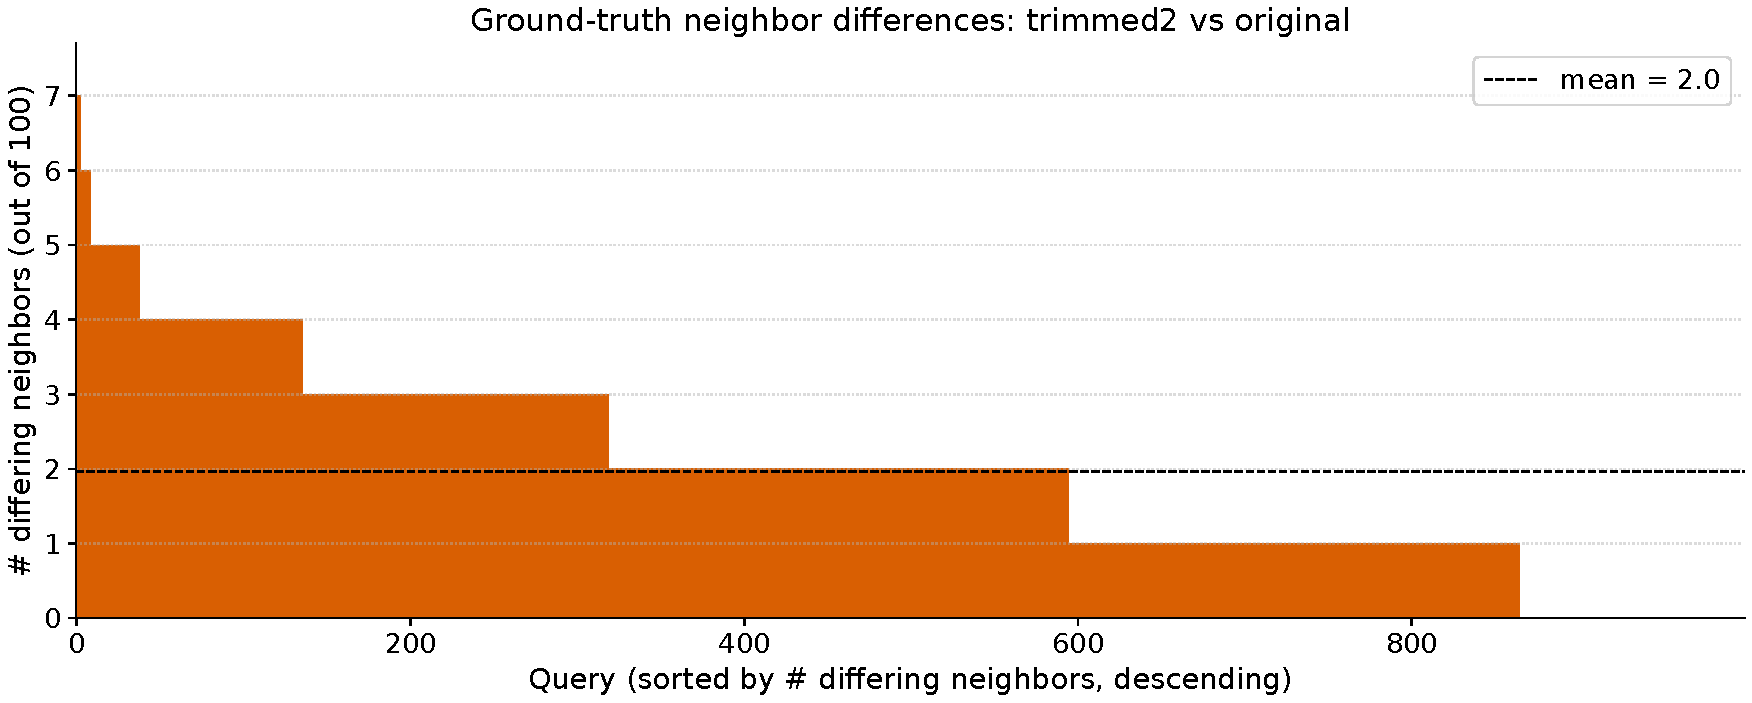
\includegraphics[width=\linewidth]{Figures/query_diff_trimmed2_vs_original.pdf}
    \caption{Per-query count of differing top-100 ground-truth neighbors
    between trimmed2 and original, sorted descending.}
    \label{fig:query-diff}
\end{figure}

Before looking at how Milvus stores the two collections on disk, we
first establish two properties of the workload that motivate asking the
question in the first place.



\mypar{Most vectors are never queried, and the accessed ones are
broadly dispersed.} \autoref{fig:hotness} plots, for each of the top-1000
most frequently accessed vectors, how many of the 1{,}000 benchmark
queries include it in their top-100 ground-truth list. The maximum
per-vector hit count is only 4 and the curve is essentially flat,
meaning no single vector is significantly hotter than any other. At the
corpus level, roughly 92\% of all vectors never appear in any query's
top-100 list, which is expected given that the benchmark returns 100
neighbors per query across approximately one million corpus vectors, so
the reachable fraction is on the order of
$100 \times 1{,}000 / 10^6 \approx 10\%$ before accounting for overlap
across queries. \autoref{fig:query-segments} then characterizes where
the touched vectors reside: for each query it counts how many of the
100 ground-truth neighbors fall into each segment of the original
collection. Neighbors are distributed across many segments per query
rather than bunched into one or two, so the ground-truth top-100 set is
broadly dispersed across the storage layout.


\mypar{The two collections answer most queries with the same neighbors.}
\autoref{fig:query-diff} compares the top-100 ground truth neighbor
lists between trimmed2 and original after remapping trimmed2 IDs into
the original index space. For the vast majority of queries the two
lists are identical or differ by only a handful of neighbors, and only
a small tail of queries sees substantial churn.
% At the workload level
% the two collections really are near-duplicates, so system that can
% align their segments has a real opportunity to serve both from shared
% data.

\subsection{Storage layout for near-identical collections}

\begin{figure*}[t]
    \centering
    \begin{subfigure}[t]{0.49\linewidth}
        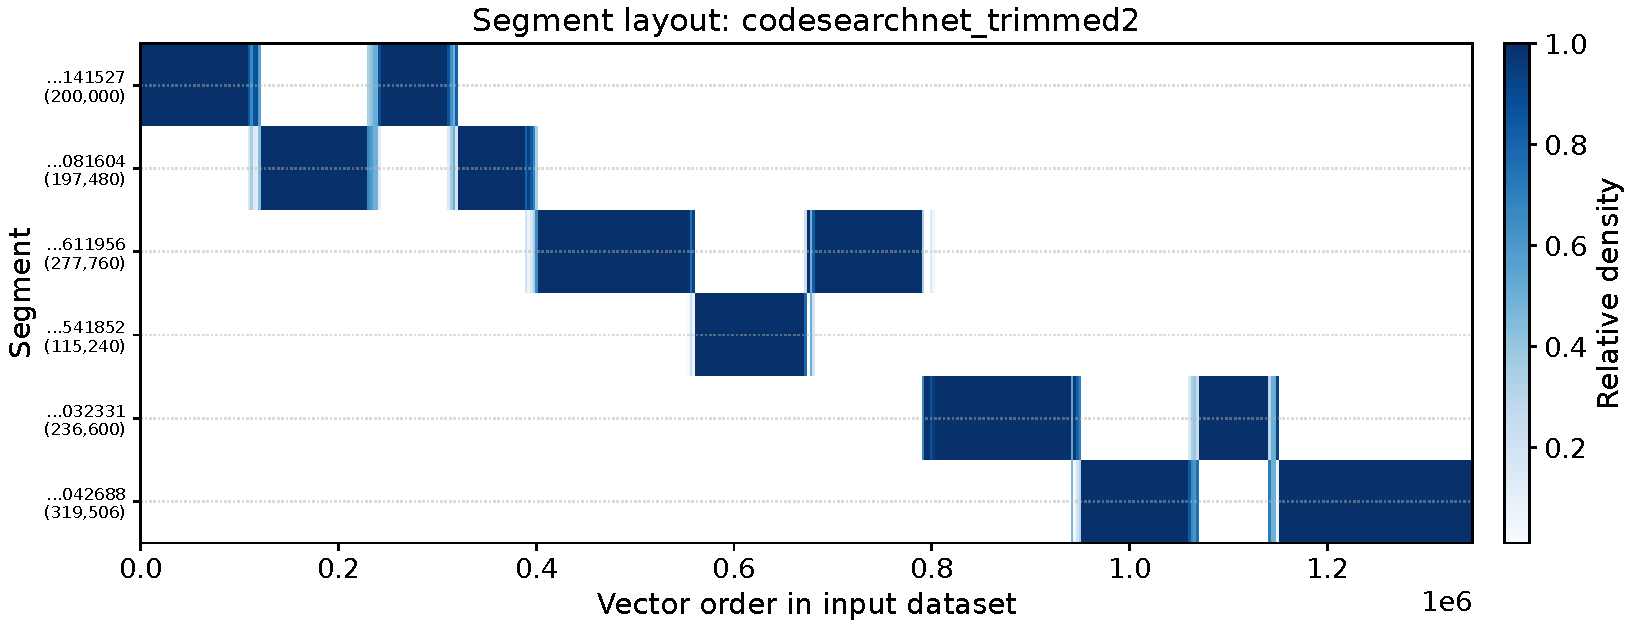
\includegraphics[width=\linewidth]{Figures/segment_layout_codesearchnet_trimmed2_bothOn.pdf}
        \caption{bothOn (stock Milvus).}
    \end{subfigure}\hfill
    \begin{subfigure}[t]{0.49\linewidth}
        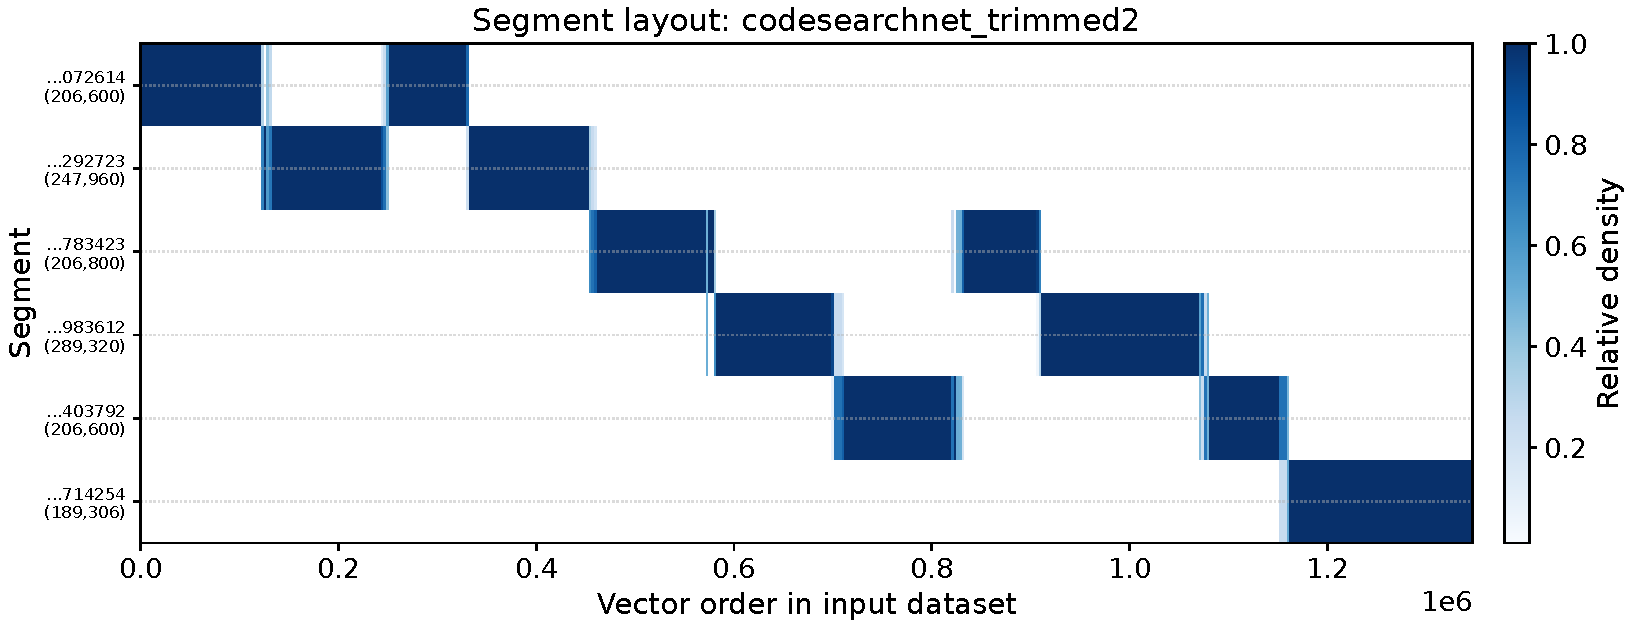
\includegraphics[width=\linewidth]{Figures/segment_layout_codesearchnet_trimmed2_nojitter.pdf}
        \caption{nojitter.}
    \end{subfigure}
    \caption{Segment layout of the trimmed2 collection. The X axis is the
    vector index in the input dataset and each row is one segment; darker
    cells indicate more vectors at that index landing in that segment.}
    \label{fig:segment-layout}
\end{figure*}

\begin{figure*}[t]
    \centering
    \begin{subfigure}[t]{0.33\linewidth}
        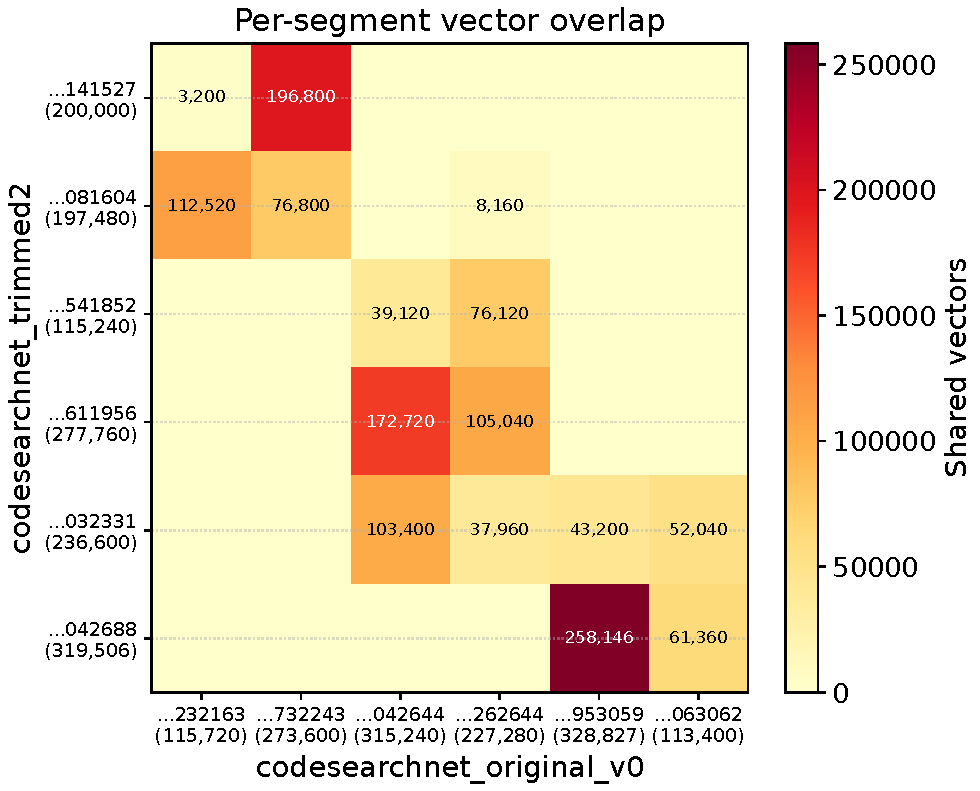
\includegraphics[width=\linewidth]{Figures/segment_overlap_codesearchnet_trimmed2_vs_codesearchnet_original_v0_bothOn.pdf}
        \caption{bothOn.}
    \end{subfigure}\hfill
    \begin{subfigure}[t]{0.33\linewidth}
        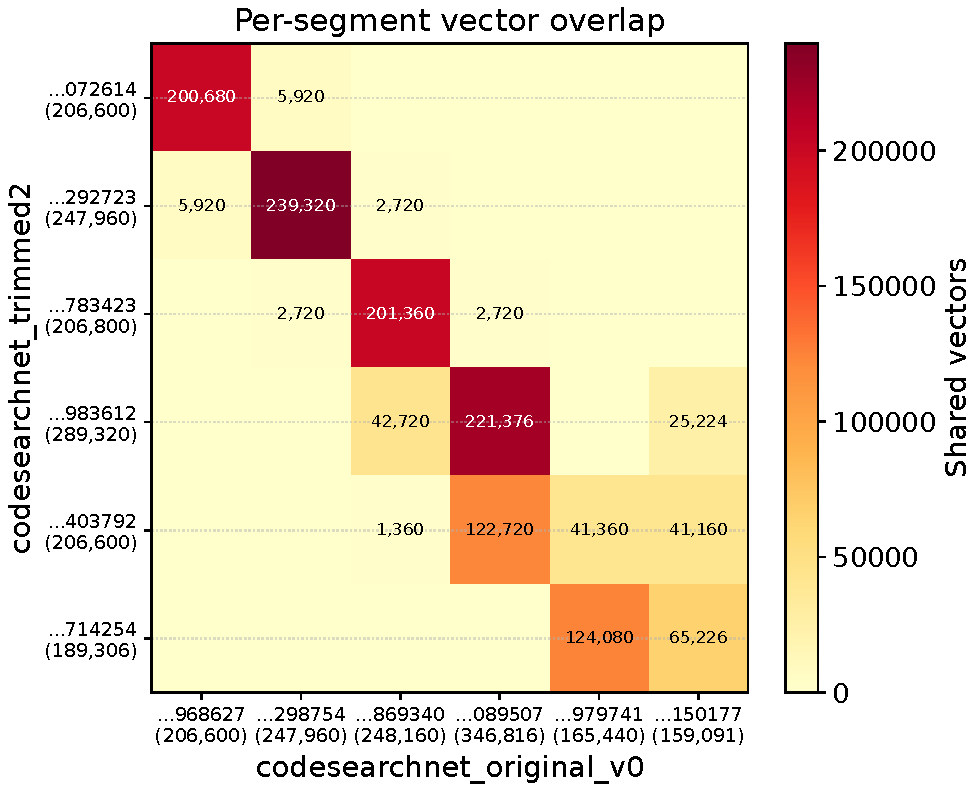
\includegraphics[width=\linewidth]{Figures/segment_overlap_codesearchnet_trimmed2_vs_codesearchnet_original_v0_nojitter.pdf}
        \caption{nojitter.}
    \end{subfigure}\hfill
    \begin{subfigure}[t]{0.31\linewidth}
        \raisebox{1.5mm}{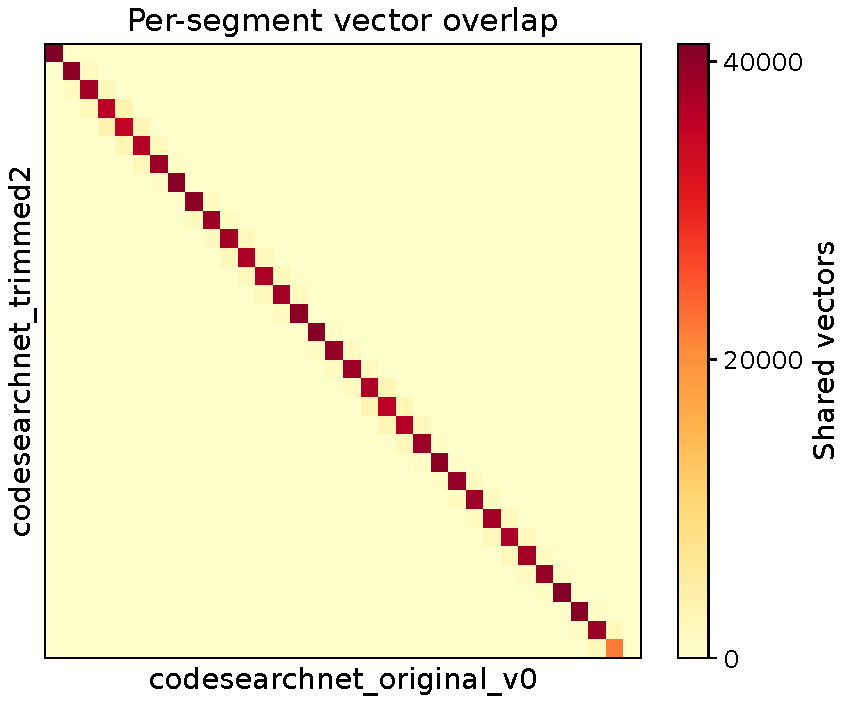
\includegraphics[width=\linewidth]{Figures/segment_overlap_codesearchnet_trimmed2_vs_codesearchnet_original_v0_noJitterCompaction.pdf}}
        \caption{noJitterCompaction.}
    \end{subfigure}
    \caption{Per-segment vector overlap between the trimmed2 and original
    collections. Rows are trimmed2 segments, columns are original segments,
    color encodes the number of shared primary keys.}
    \label{fig:segment-overlap}
\end{figure*}

Given a workload where the two collections are near-duplicates at the
query level, we now ask how Milvus~\cite{wang2021milvus} actually lays
them out on disk. Milvus organizes a collection as a sequence of
segments that are flushed from a write-ahead buffer, and a background
compactor may later merge small segments~\cite{guo2022manu}.

\mypar{Compaction, not jitter, is the main source of non-contiguous
segments.} \autoref{fig:segment-layout} shows, for the trimmed2
collection, which vector ranges of the input dataset end up in each
segment. Neither configuration produces a clean staircase. Under stock
Milvus (bothOn), each segment covers several disjoint bands of the
input vector space, and the bands themselves are smeared because the
jittered flush size makes different flushes seal at different vector
counts. Disabling jitter (nojitter) makes each band somewhat cleaner, but a
single segment still draws from two or more such strips, so even
without jitter the vector ranges held by a segment
are not contiguous. The reason is that compaction is still running:
the background compactor merges earlier-flushed segments into new
ones, and because those earlier segments were themselves flushed at
different points in the insert stream, the merged segment ends up
holding vectors from multiple non-adjacent input ranges. Jitter therefore
controls only the fuzziness of each strip, whereas the gap between the
two strips that share a segment is controlled by compaction.

\mypar{Cross-collection overlap is only meaningful under
noJitterCompaction.} \autoref{fig:segment-overlap} shows the
per-segment overlap matrix between the trimmed2 and original
collections for each of the three configurations. Each cell records the
number of vectors that a segment in trimmed2 (row) shares with a
segment in original (column). With stock Milvus, the matrix is dense
and scattered: shared vectors are smeared across many segment pairs, so
picking any single segment of the second collection only recovers a
small fraction of the vectors that a segment of the first holds. The
scatter is amplified by how jitter interacts with compaction: Milvus
selects which small segments to merge based on their sizes, and because
jitter produces differently sized segments across the two collections,
the compactor makes different merging choices for each, further
diverging their segment boundaries even when the underlying data is
nearly identical. Disabling jitter helps because it makes the first several compaction
choices identical across the two collections, which narrows each band
in the overlap matrix. However, as the number of remaining small
segments shrinks and their sizes approach the merge threshold, the
compactor's size-based selection hits a boundary where a small
difference tips the choice of which segments to merge, so the matrix
is still noisy in the nojitter configuration. With noJitterCompaction the overlap
collapses to a near-diagonal structure, where each trimmed2 segment has
one matching original segment and the shared region accounts for the
bulk of its vectors. The small offset along the diagonal is exactly the
2\% of vectors trimmed2 dropped from the head of the corpus. We also ran
the same comparison for two independent copies of the original
collection
% (\texttt{original\_v0} vs \texttt{original\_v1}) 
 and got
qualitatively identical behavior, which means the shuffling is inherent
to Milvus's ingest path and not specific to the trimmed workload.

\subsection{Storing in partitions within one collection}

\begin{figure}[t]
    \centering
    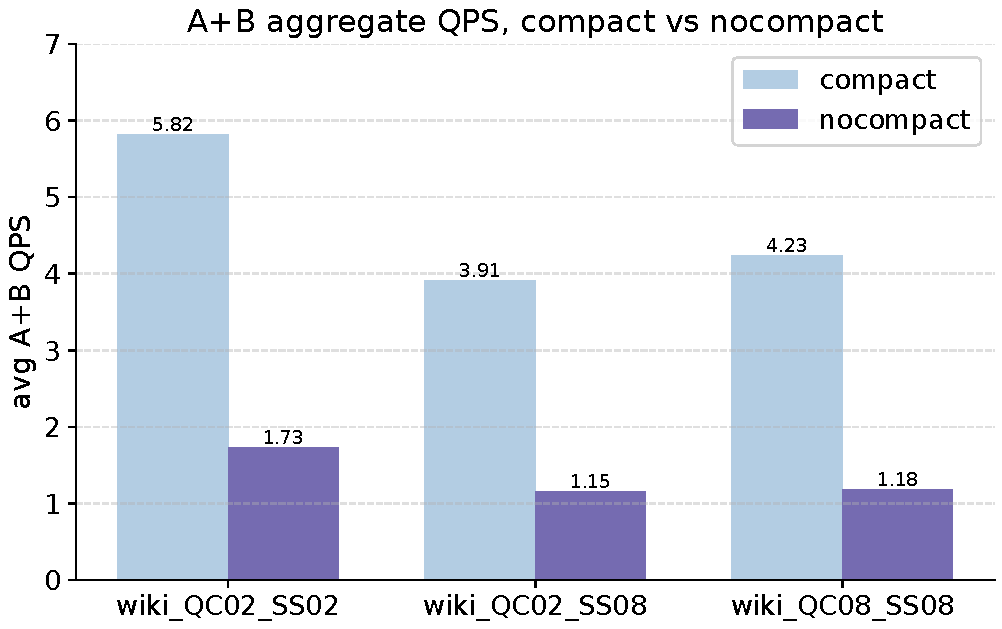
\includegraphics[width=\linewidth]{Figures/qps_compact_vs_nocompact.pdf}
    \caption{Aggregate $A$+$B$ concurrent QPS for the three Wikipedia
    workload variants, with compaction enabled and disabled.
    Compaction yields a roughly $3\times$ improvement across all
    variants.}
    \label{fig:qps-compact-vs-nocompact}
\end{figure}

\begin{figure}[t]
    \centering
    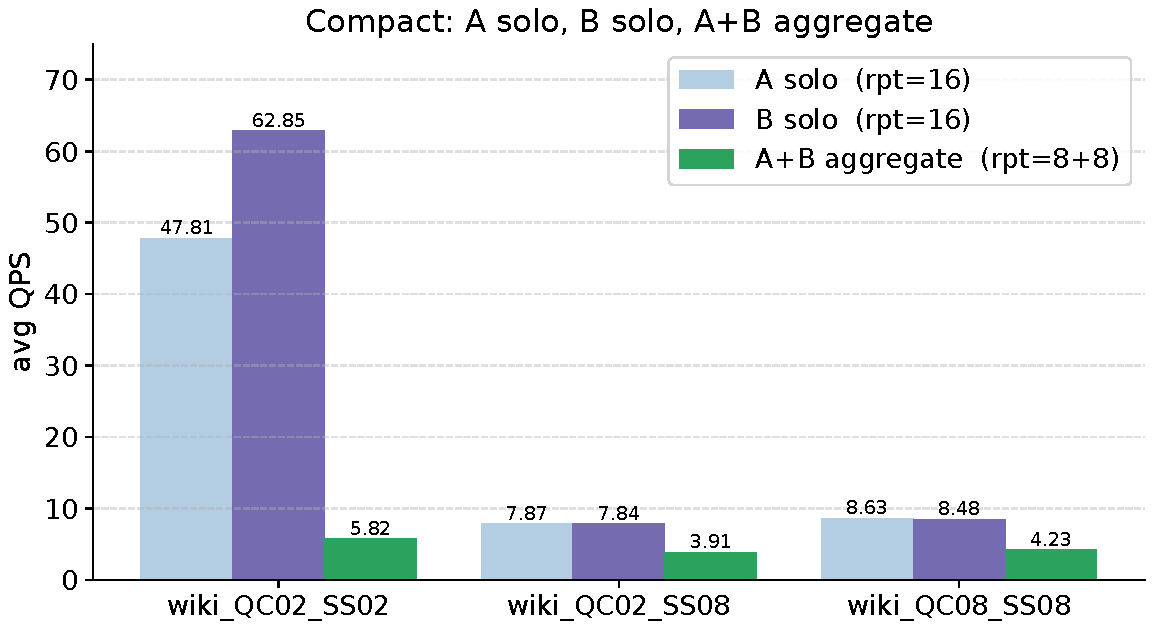
\includegraphics[width=\linewidth]{Figures/qps_compact_solo_vs_concurrent.pdf}
    \caption{Solo per-tenant QPS versus aggregate concurrent QPS on
    each compacted variant. On QC02\_SS02 the gap between solo and
    concurrent throughput exceeds an order of magnitude, while the
    QC*\_SS08 variants are already disk-bound in the solo case.}
    \label{fig:qps-solo-vs-concurrent}
\end{figure}

\begin{figure}[t]
    \centering
    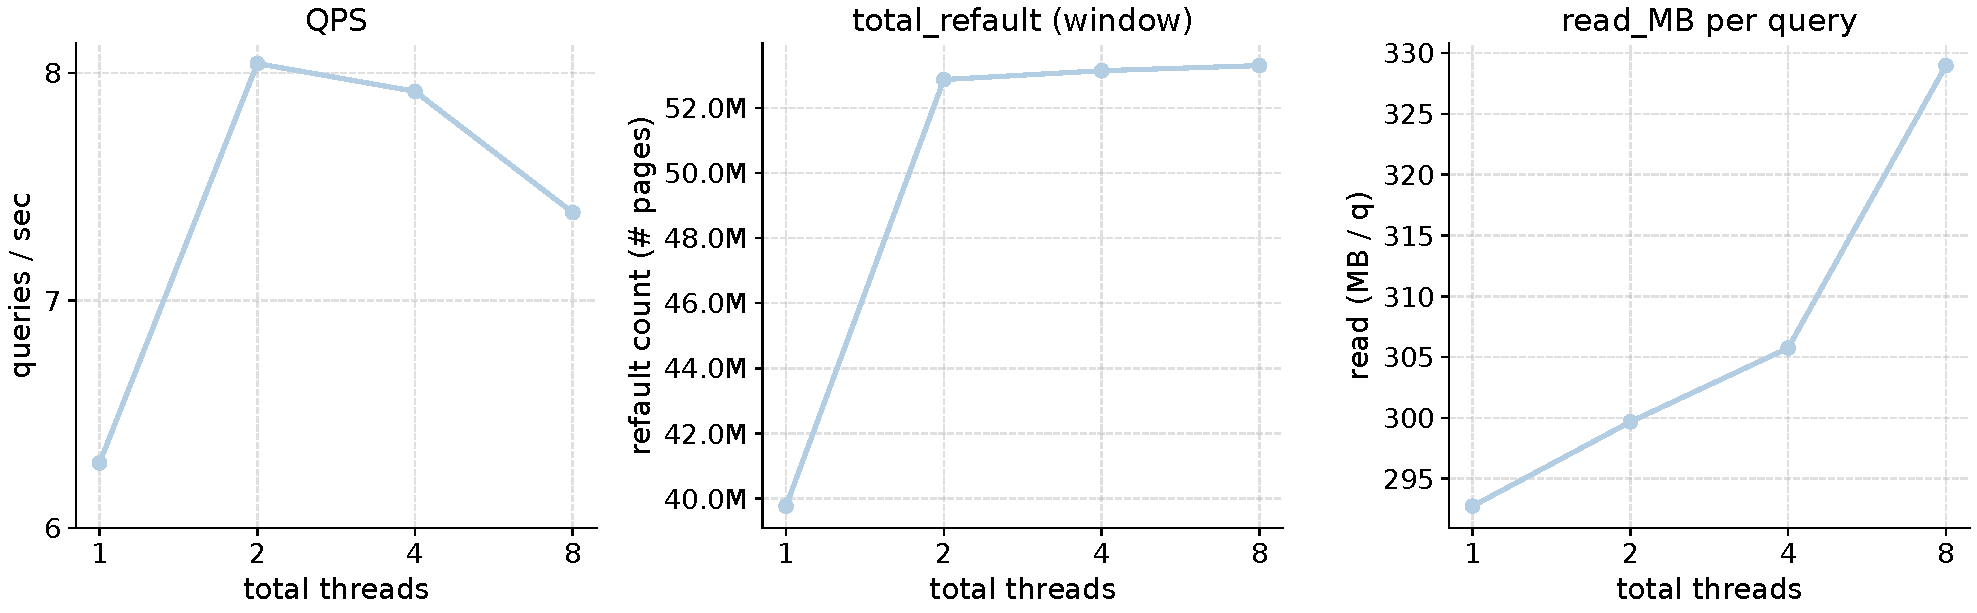
\includegraphics[width=\linewidth]{Figures/cache_miss_metrics_wiki_QC02_SS08.pdf}
    \caption{QPS, major page faults, and read volume per query as a
    function of total query threads on QC02\_SS08\_nocompact. Stable
    refault counts paired with rising per-query reads and falling QPS
    are the signature of page-cache thrashing.}
    \label{fig:cache-miss-metrics}
\end{figure}

The shared partition layout removes the storage redundancy of the
fully replicated layout by keeping a single collection in which the
shared corpus and each tenant's private vectors live in distinct
partitions. The open question for this layout is whether the
resulting resource sharing translates into competitive query
throughput once tenants query their respective tenant partitions
concurrently. We measure throughput along two axes: the effect of
compaction on aggregate concurrent throughput, and the per-tenant
throughput under solo and concurrent execution. We then drill into
a single configuration to identify the bottleneck that limits
concurrent performance.

\mypar{Compaction roughly triples aggregate throughput.} For each of
the three Wikipedia workload variants, we issue queries from both
tenants concurrently and report the aggregate QPS of $A$ and $B$
combined in \autoref{fig:qps-compact-vs-nocompact}. With compaction
enabled, the aggregate throughput is 5.82, 3.91, and 4.23 QPS for
QC02\_SS02, QC02\_SS08, and QC08\_SS08 respectively. Disabling
compaction drops the same numbers to 1.73, 1.15, and 1.18 QPS, a
factor of roughly $3\times$ across all three variants. The mechanism is straightforward: compaction merges many
small sealed segments into a smaller number of larger ones, so each
query fans out to fewer segments at search time and the working set
spans fewer page-cache pages. The compaction-disabled collections,
which carry roughly three times as many segments at the same total
vector count, force every query to scan more index files and pull more
pages off disk per request.

\mypar{Concurrent execution collapses solo throughput by an order of
magnitude.} \autoref{fig:qps-solo-vs-concurrent} contrasts each
tenant's solo throughput with the aggregate concurrent throughput on
the compacted collections. On QC02\_SS02 tenant $A$ alone reaches
47.81~QPS and tenant $B$ alone reaches 62.85~QPS, but running both
tenants concurrently yields a combined throughput of only 5.82~QPS,
roughly an order of magnitude below either solo case. The reason is
that QC02\_SS02 places 14.2M vectors in each tenant partition, and the
per-tenant working set comfortably fits in the 96\,GB RAM cap when
only one tenant is active. Once the second tenant joins and brings
its own 14.2M vector partition into active rotation, the combined
working set overflows the RAM cap and the page cache begins evicting
pages that the first tenant will read again on its next query. On
the two QC*\_SS08 variants, where 80\% of cold vectors live in the
shared partition and the tenant partitions are only 3.7 to 3.9M
vectors, solo throughput is already low at roughly 8~QPS because each
query must traverse the much larger shared partition, and even a
small tenant partition is enough to halve concurrent throughput once
both tenants are active. Whether a query could in principle be
answered entirely within the shared partition or entirely within
its tenant partition does not change the throughput observed on the
QC*\_SS08 variants, because the current search path is content
agnostic: every query fans out to all segments in the shared
partition and in its tenant partition, scans each one, and merges
the results, regardless of where the actual top-$k$ neighbors
reside. As a result, QC02\_SS08 and QC08\_SS08, which differ only
in how concentrated the top-$k$ neighbors are inside the shared
partition, exhibit essentially the same throughput under
concurrent execution.

\mypar{Scalability is bounded by page-cache thrashing, not CPU.} To
pin down the bottleneck, we sweep the number of query threads issued
against tenant $A$ on the QC02\_SS08\_nocompact collection, whose
relevant partition set comprises 240 segments, and track QPS, major
page fault count, and read volume per query as shown in
\autoref{fig:cache-miss-metrics}. QPS rises from 5.5~q/s at one
thread to 8.1~q/s at two threads, then \emph{falls} to 7.3~q/s at
eight threads, so adding concurrent requests actively reduces
throughput rather than scaling the system. The major page
fault count plateaus at roughly 53M pages across two, four, and
eight threads, indicating that the disk page-read rate is saturated
and is the binding ceiling rather than the CPU. The total read
volume per query, in contrast, keeps climbing from 293\,MB at one
thread to 329\,MB at eight threads, because each query increasingly
re-reads pages that a different concurrent query has just evicted
from the page cache. Stable refault counts, rising per-query read
volume, and falling QPS together form the classical signature of
page-cache thrashing, and they confirm that the shared partition
layout's performance ceiling under concurrency is dictated by how
the segment-level working set interacts with the page cache rather
than by the cost of index search itself.
